\section{JPA: entity manager}

The entity instances are plain Java objects, and for this reason they not become managed until the application invokes an API method to initiate the process. The
entity manager is the central authority for all persistence actions. In particular, it manages the mapping and APIs for interacting with the database and the objects. 
\begin{definition}
    The \emph{persistence context} is the fundamental and exclusive concept of Java Persistence API: it is a kind of main memory database that holds the objects in 
    the managed state. 
\end{definition}
A managed object is tracked, so all the modifications to its state are monitored for automatic alignment to the database. 
Database writes by default occur asynchronously, and when they happen the persistence context must hook up to a transaction. So, we have that a managed entity has two 
lives: one as a Java object and one as a relational tuple bound to it. Such a binding exists only inside the persistence context. When the POJO exits the persistence 
context the binding breaks: it gets untracked and no longer synchronized to the database. Note that the application never sees the persistence context, it interacts
only with the entity manager.

\subsection*{Interface}
The interface of the entity manages exposes the following methods: 
\begin{itemize}
    \item Makes an entity instance become part of the persistence context. 
        \begin{lstlisting}[style=Java]
public void persist(Object entity); 
        \end{lstlisting}
    \item Finds an entity instance by its primary key. 
        \begin{lstlisting}[style=Java]
public <T> T find(Class<T> entityClass, Object primaryKey);
        \end{lstlisting}
    \item Removes an entity instance from the persistence context and thus from the database.
        \begin{lstlisting}[style=Java]
public void remove(Object entity); 
        \end{lstlisting}
    \item Resets the state of entity instance from the content of the database.
        \begin{lstlisting}[style=Java]
public void refresh(Object entity); 
        \end{lstlisting}
    \item Writes the state of entities to the database as immediately as possible.
        \begin{lstlisting}[style=Java]
public void flush();
        \end{lstlisting}
\end{itemize}
When an entity is first instantiated, it is in the transient state since the entity manager does not know it exists yet. Transient entities are not part of the 
persistence context associated with the entity manager. 
\begin{example}
    A new POJO can be created in the following way: 
    \begin{lstlisting}[style=Java]
Employee emp = new Employee(ID, "John Doe"); 
    \end{lstlisting}
\end{example}
To make the transient entities managed we have to use the method persist() of the entity manager. Note that when an entity becomes managed, all the changes apply to it 
will apply also to the database itself, and the other way round. The managed entity and the corresponding tuple become associated until the entity exits the managed state. It is 
possible to call persist() on a managed entity: this will trigger the cascade process. 
\begin{example}
    A new POJO can be created and later made managed in the following way: 
    \begin{lstlisting}[style=Java]
Employee emp = new Employee(ID, "John Doe"); 
em.persist(emp);
    \end{lstlisting}
\end{example}
We can find an entity with find() method. It  takes as an input the class of the entity that is being sought and the primary key value that identifies the desired 
entity instance. When the call completes, the returned object will be managed. If the entity instance is not found, then the find() method returns null. 
\begin{example}
    Finding an entity
    \begin{lstlisting}[style=Java]
Employee emp = em.find(Employee.class, ID);
    \end{lstlisting}
\end{example}
We can remove an entity with remove() method. It breaks the association between the entity and the persistence context. When the transaction associated with the 
entity manager's persistence context commits or the entity manager flush() method is called, the tuple associated with the entity is scheduled for deletion from
the database. The entity still exists, but its changes are no longer tracked for being synchronized to the database.
\begin{example}
    Removing an entity
    \begin{lstlisting}[style=Java]
em.remove(emp);
    \end{lstlisting}
\end{example}

\begin{figure}[H]
    \centering
    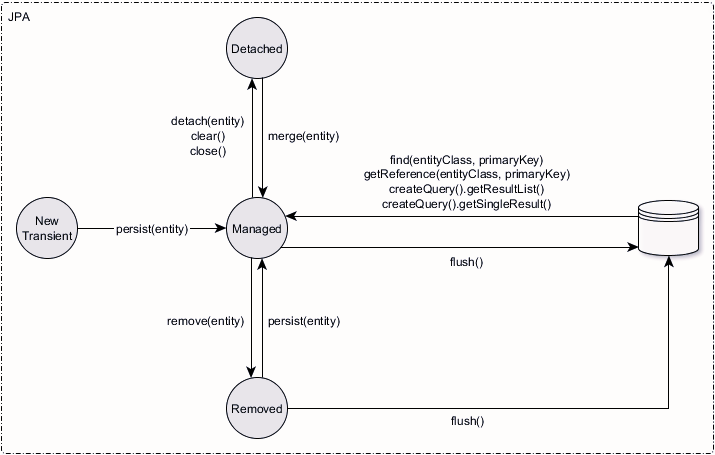
\includegraphics[width=0.75\linewidth]{images/jpaem.png}
    \caption{Possible states for the entities}
\end{figure}
According to the previous graph we have that an entity can be in five main states (deleted is omitted in the image): 
\begin{itemize}
    \item New: the entity is unknown to the entity manager, has no persistent identity, and has no tuple associated. 
    \item Managed: the entity is associated with persistence context, changes to objects automatically, and synchronizes to database. 
    \item Detached: the entity has an identity potentially associated with a database tuple, but changes are not automatically propagated to the database.
    \item Removed: the entity is scheduled for removal from the database.
    \item Deleted: the entity is erased from the database. 
\end{itemize}

\subsection*{Application architecture}
In Java Enterprise Edition the client exploits the services the EJB container to connect to the entity manager. In particular, the business level interacts with 
the entity manager. The advantage of the EJB is that this container provides the support to make JPA entity method calls transactional through the automatic creation 
of transactions. 
\begin{figure}[H]
    \centering
    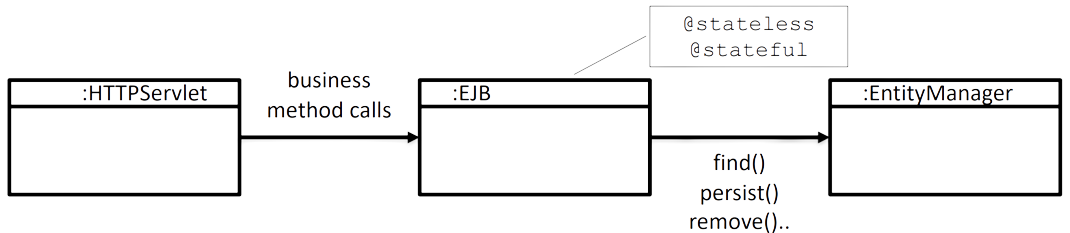
\includegraphics[width=0.75\linewidth]{images/jee1.png}
\end{figure}
The transactions exist at three levels: 
\begin{itemize}
    \item DBMS transactions: they are managed by the DBMS and use SQL. 
    \item Resource-local transactions: they are managed by the application and use the JDBC connection interface. They are mapped to the JDBC. 
    \item Container transaction: they are managed by the application or the container and use the JTA interface. They are mapped to the JDBC. 
\end{itemize}
The level used by the entity manager is the container transaction one. After defining a business object, the container injects the entity manager into it. The 
container manages instances of the entity manager transparently to the application. The container provides the transaction needed for saving the modifications made 
to the entities of the persistence context associated with the entity manager into the database. 
\begin{example}
    Definition of a business object EJB: 
    \begin{lstlisting}[style=Java]
@Stateless 
public class myEJBService {
@PersistenceContext(unitName = "MyPersistenceUnit")
private EntityManager em; 
}
    \end{lstlisting}
\end{example}
When a client calls a method of a business object that exploits a container managed entity manager for persistence, the container provides a transaction for saving 
the modifications to the database (if the same transaction is called multiple times it will be reused). Note that this is the most common and default behavior, but 
the business objects methods can be annotated to specify a different way to use the transactions provided by the container. A method can be annotated to obtain the 
desired transactional behaviour with @TransactionAttribute(TransactionAttributeType.type), where type can be: 
\begin{itemize}
    \item Mandatory: a transaction is expected to have already been started and be active when the method is called. If no transaction is active, an exception is thrown.
    \item Required: the default, if no transaction is active one is started. If one is active this is used.
    \item Requires$\_$new: the method always needs to be in its own transaction. Any active transaction is suspended. 
    \item Supports: the method does not access transactional resources, but tolerates running inside one if it exists.
    \item Not$\_$supported: the method will cause the container to suspend the current transaction if one is active when the method is called. 
    \item Never: the method will cause the container to throw an exception if a transaction is active when the method is called.
\end{itemize}